% !TEX program = xelatex
% !TEX options = --shell-escape
\documentclass[a4paper,9]{article}
\usepackage{zh_CN-Adobefonts_external} % Simplified Chinese Support using external fonts (./fonts/zh_CN-Adobe/)
\usepackage{fancyhdr}
\usepackage[cache=false]{minted}
\usemintedstyle{bw}
\usepackage[colorlinks]{hyperref}
\setlength{\headheight}{15pt}
\usepackage{geometry}
\usepackage{amsmath,amssymb,bm}
\usepackage{pdfpages}
\usepackage{ulem}

% 定义页边距
\geometry{a4paper,left=1cm,right=1cm,top=2cm,bottom=2cm}

% 定义页眉页脚
\pagestyle{fancy}
\fancyhf{}
\fancyhead[C]{Algorithm Library, yet to be explored, lcy}
\lfoot{}
\cfoot{\thepage}
\rfoot{}

\author{
Shanghai Jiao Tong University\\
\vspace{0cm}\\
\Large{\textit{未至之境}}\\
\Large{\textit{Yet to be Explored}}\\
\vspace{0cm}\\
Chengyuan Luo}
\title{Algorithm Library}
\date{November, 2021\\
\small{\vspace{0.4cm}The template of these templates is based on \href{https://github.com/palayutm/ply-template}{palayutm/ply-template}\\
Some of the codes are taken from:\\
\href{https://github.com/FTRobbin/Dreadnought-Standard-Code-Library}
{FTRobbin/Dreadnought-Standard-Code-Library},\\
\href{https://github.com/laonahongchen/ICPC-code-template-Quasar-}
{laonahongchen/ICPC-code-template-Quasar-},\\
\href{https://github.com/laonahongchen/ICPC-code-template-Blazar}
{laonahongchen/ICPC-code-template-Blazar}.
}}

\begin{document}

\twocolumn  % 分页显示

\maketitle % 封面
% \newpage % 换页
\begingroup
\hypersetup{linkcolor=black}
\tableofcontents % 目录
\endgroup

\section{Vim 配置}
\subsection{vimrc}
\inputminted[breaklines]{vim}{source/vimrc/vimrc}
\subsection{VS Code}
\inputminted[breaklines]{json}{source/vimrc/vscode.json}

\section{Z}
\inputminted[breaklines]{c++}{source/Z/Z.cpp} % 插入代码文件

\section{随机数生成器}
\inputminted[breaklines,breakanywhere]{c++}{source/random/rand-gen.cpp}

\section{数列与计数}
\subsection{多项式板子}
\inputminted[breaklines]{c++}{source/sequence/polynomial.cpp}
\subsection{牛顿迭代}
\noindent \textbf{问题描述:}给出多项式$G(x)$,求解多项式$F(x)$满足:
\[G(F(x)) \equiv 0 \pmod {x^n}\]
答案只需要精确到$F(x) \bmod {x^n}$即可。\par
\noindent \textbf{实现原理:}考虑倍增,假设有:
\[G(F_t(x)) \equiv 0 \pmod{x^t}\]
对$G(F_{t + 1}(x))$在模$x^{2t}$意义下进行Taylor展开:
\[G(F_{t + 1}(x)) \equiv G(F_t(x)) + \dfrac{G'(F_t(x))}{1!}(F_{t + 1}(x) - F_t(x)) \pmod{x^{2t}}\]
那么就有:
\[F_{t + 1}(x) \equiv F_t(x) - \dfrac{G(F_t(x))}{G'(F_t(x))} \pmod{x^{2t}}\]
\noindent \textbf{注意事项:}$G(F(x))$的常数项系数必然为0,这个可以作为求解的
初始条件。
\par
\noindent \textbf{多项式求逆}
\noindent \textbf{原理:}令$G(x) = x * A - 1$(其中$A$是一个多项式系数),根据牛顿迭代法有:
\begin{displaymath}
\begin{split}
F_{t + 1}(x) &\equiv F_t(x) - \dfrac{F_t(x) * A(x) - 1}{A(x)} \\
&\equiv 2F_t(x) - F_t(x)^2 * A(x)\pmod{x^{2t}}
\end{split}
\end{displaymath}
\noindent \textbf{注意事项:}
\begin{enumerate}
	\item $F(x)$的常数项系数必然不为0,否则没有逆元;
	\item 复杂度是$O(n \log n)$但是常数比较大($10^5$大概需要0.3秒左右);
	\item 传入的两个数组必须不同,但传入的次数界没有必要是2的次幂;
\end{enumerate}
\textbf{多项式取指数和对数}
\noindent \textbf{作用:}给出一个多项式$A(x)$,求一个多项式$F(x)$满足$e^A(x) - F(x) \equiv 0 \pmod{x^n}$。\par
\noindent \textbf{原理:}令$G(x) = \ln x - A$(其中$A$是一个多项式系数),根据牛顿迭代法有:
\[F_{t + 1}(x) \equiv F_t(x) - F_t(x)(\ln {F_t(x)} - A(x)) \pmod{x^{2t}}\]
求$\ln {F_t(x)}$可以用先求导再积分的办法,即:
\[\ln A(x) = \int \dfrac{F'(x)}{F(x)}~\mathrm{d}x\]
多项式的求导和积分可以在$O(n)$的时间内完成,因此总复杂度为$O(n \log n)$。\par
\noindent \textbf{应用:}加速多项式快速幂。\par
\noindent \textbf{注意事项:}
\begin{enumerate}
	\item 进行$\log$的多项式必须保证常数项系数为1,否则必须要先求出$\log a[0]$是多少;
	\item 传入的两个数组必须不同,但传入的次数界没有必要是2的次幂;
	\item 常数比较大,$10^5$的数据求指数和对数分别需要0.37s和0.85s左右的时间,注意这里{memset}几乎不占用时。
\end{enumerate}

\subsection{MTT}
\inputminted[breaklines]{c++}{source/sequence/mtt.cpp}
\subsection{FWT}
\inputminted[breaklines]{c++}{source/sequence/fwt.cpp}
\subsection{BM}
\inputminted[breaklines]{c++}{source/sequence/bm.cpp}
\subsection{numbers}
\subsubsection{伯努利数}
\noindent 伯努利数满足
\begin{equation*}
    B_0 = 1, \sum_{j=0}^m \binom{m+1}{j} B_j = 0 ~ (m > 0).
\end{equation*}
\noindent 等式两边同时加上 $B_{m+1}$,并设 $n = m - 1$,得
\begin{equation*}
\sum_{i=0}^n \binom{n}{i} B_i = [n = 1] + B_n
\end{equation*}
\noindent 设 $\hat{B}(x) = \sum_{i=0}^\infty B_i \cdot \frac{x^i}{i!}$,则
\begin{equation*}
\hat{B}(x) e^x = x + \hat{B}(x) \Rightarrow \hat{B}(x) = \frac{x}{e^x - 1} \\
\end{equation*}
\begin{equation*}
\begin{aligned}
& 0^k + 1^k + \ldots + n^k \\
=& ~ k! \left[ x^k \right] \frac{e^{(n+1)x}-1}{x} \cdot \hat{B}(x) \\
=& ~ k! \sum_{i=0}^k \frac{B_i}{i!} \cdot \frac{(n+1)^{k-i+1}}{(k-i+1)!} \\
=& ~ \frac{1}{k+1} \sum_{i=0}^k \binom{k+1}{i} B_i \cdot (n+1)^{k-i+1}
\end{aligned}
\end{equation*}

\subsubsection{第一类斯特林数}
\noindent 记 $S_1(n, k)$ 为将 $n$ 个不同元素分为 $k$ 个环排列的方案数. 由组合意义得,
$$
S_1(n, k) = S_1(n - 1, k - 1) + (n - 1) S_1(n - 1, k)
$$
$$
x^{\overline{n}} = \sum_{i=0}^n S_1(n, i) x^i
$$
$$
x^{\underline{n}} = \sum_{i=0}^n (-1)^{n-i} S_1(n, i) x^i
$$
$$
\sum_{i=0}^n S_1(n, i) x^i = \prod_{i=0}^{n-1} (x+i)
$$

\noindent 注意最后等式的右半部分,可以使用递增 + 点值平移 $O(n \log n)$ 求出第
$n$ 行斯特林数.

\subsubsection{第二类斯特林数}
\noindent 记 $S_2(n, k)$ 为将 $n$ 个不同元素分至 $k$ 个相同的盒子(每个盒子至
少一个元素)的方案数. 由组合意义得,
$$
S_2(n, k) = S_2(n - 1, k - 1) + k S_2(n - 1, k)
$$
$$
x^n = \sum_{i=0}^n S_2(n, i) x^{\underline{i}}
$$
$$
S_2(n, k) = \sum_{i=0}^k (-1)^{k-i} \binom{k}{i} i^n
$$
$$
\frac{S_2(n, k)}{k!} = \sum_{i=0}^k \frac{i^n}{i!} \cdot \frac{(-1)^{k-i}}
{(k-i)!}
$$
\noindent 是一个卷积的形式,可以 FFT 求出某一行第二类斯特林数.

\subsubsection{斯特林反演}
\begin{equation*}
    \begin{aligned}
        x^n &= \sum_{i=0}^n S_2(n, i) x^{\underline{i}} \\
        &= \sum_{i=0}^n S_2(n, i) \sum_{j=0}^i (-1)^{i-j} S_1(i, j) x^j \\
        &= \sum_{i=0}^n x^i \sum_{j=i}^n (-1)^{j-i} S_2(n, j) S_1(j, i)
    \end{aligned}
\end{equation*}
\noindent 设
\begin{equation*}
    g_n = \sum_{i=0}^n S_2(n, i) f_i,
\end{equation*}
\noindent 则
\begin{equation*}
    f_n = \sum_{i=0}^n (-1)^{n-i} S_1(n, i) g_i.
\end{equation*}

\subsubsection{Burnside 引理}
\hspace{\parindent}设置换群为 $G$,染色集合为 $X$.

若染色 $x \in X$ 在置换 $f$ 的作用下得到染色 $y \in X$,则称 $x, y$ 等价.
由置换群的定义,我们可以得到等价类,使得等价类内任意两个染色等价.

设 $X^g (g \in G)$ 表示在置换 $g$ 下的不动点,即
$$
X^g = \{x \mid x \in X, gx = x\}.
$$
则等价类个数
$$
|X / G| = \frac{1}{|G|} \sum_{g \in G} |X^g|.
$$

例 LOJ 6538 烷基计数,对于一棵有根树,每个节点至多三个儿子,且这些儿子排列同
构. 求有多少个 $n$ 个节点的等价类.

考虑其生成函数 $f(x)$.
根节点有 $3$ 个儿子(儿子可以为空,因为循环同构,我们不需讨论 $0, 1, 2$ 个儿子
的情况),排列的置换群有 $6$ 种,其中 $(1,2,3)$ 染色方案数为 $f(x)^3$,
$(1,3,2),(2,1,3),(3,2,1)$ 染色方案为 $f(x^2)f(x)$,$(2,3,1),(3,1,2)$ 染色方案
为 $f(x^3)$. 所以
$$
f(x) = x \times \frac{f(x)^3+3f(x^2)f(x)+2f(x^3)}{6}+1.
$$
牛顿迭代.

\subsubsection{五边形数}
$
    \prod_{n=1}^{\infty}{(1-x^{n})}=\sum_{n=0}^{\infty}{(-1)^{n}(1-x^{2n+1})x^{n(3n+1)/2}}
$

\subsection{树的计数}
\begin{enumerate}
	\item 有根树计数:$n+1$个结点的有根树的个数为
	$$a_{n+1} = \frac{\sum_{j=1}^{n}{j \cdot a_j \cdot{S_{n, j}}}}{n}$$
	其中,
	$$S_{n, j} = \sum_{i=1}^{n/j}{a_{n+1-ij}} = S_{n-j, j} + a_{n+1-j}$$
	\item 无根树计数:当$n$为奇数时,$n$个结点的无根树的个数为
	$$a_n-\sum_{i=1}^{n/2}{a_ia_{n-i}}$$
	当$n$为偶数时,$n$个结点的无根树的个数为
	$$a_n-\sum_{i=1}^{n/2}{a_ia_{n-i}}+\frac{1}{2}a_{\frac{n}{2}}(a_{\frac{n}{2}}+1)$$
	\item $n$个结点的完全图的生成树个数为
	$$n^{n-2}$$
	\item 矩阵-树定理:图$G$由$n$个结点构成,设$\bm{A}[G]$为图$G$的邻接矩阵、$\bm{D}[G]$为图$G$的度数矩阵,则图$G$的不同生成树的个数为$\bm{C}[G] = \bm{D}[G] - \bm{A}[G]$的任意一个$n-1$阶主子式的行列式值。
\end{enumerate}



\section{数论}
\subsection{判素数(miller-rabin)}
\inputminted[breaklines]{c++}{source/number-theory/miller_rabin.cpp}
\subsection{二次剩余(Cipolla)}
欧拉判定:
\begin{equation*}
    x^{\frac{p-1}{2}} \equiv \binom{\underline{x}}{p} \pmod p
\end{equation*}

\inputminted[breaklines]{c++}{source/number-theory/cipolla.cpp}
\subsection{杜教筛}
\inputminted[breaklines]{c++}{source/number-theory/dujiaoshai.cpp}
\subsection{min\_25}
\inputminted[breaklines]{c++}{source/number-theory/min25.cpp}
\subsection{佩尔方程}
\inputminted[breaklines]{c++}{source/number-theory/pell.cpp}
\subsection{直线下整点个数}
\inputminted[breaklines]{c++}{source/number-theory/lattice_count.cpp}
\subsection{定理}
\subsubsection{扩展欧拉定理}
\begin{equation*}
    a^b \equiv \begin{cases} a^{b \bmod \varphi(m)} & (\gcd(a, m) = 1) \\ a^b & (\gcd(a, m) \ne 1, b < \varphi(m)) \\ a^{(b \bmod \varphi(m)) + \varphi(m)} & (\gcd(a, m) \ne 1, b \ge \varphi(m)) \end{cases} \pmod m
\end{equation*}

\subsubsection{卢卡斯定理}
\noindent $\forall$ 质数 $p, n, m \in \mathbb{N}^{+}$,
\begin{equation*}
    \binom{n}{m} \equiv \binom{\lfloor n/p \rfloor}{\lfloor m/p \rfloor}
    \binom{n \bmod p}{m \bmod p} \pmod p
\end{equation*}

\subsubsection{威尔逊定理}
\noindent 对于质数 $p$,有 $(p-1)! \equiv -1 \pmod p$(证明 $2, 3, \ldots, p -
2$ 可以逆元两两配对)
\noindent 高斯的扩展:
\begin{equation*}
    \prod_{1 \le k \le m, \gcd(k, m) = 1} k \equiv \begin{cases} -1, &
    \text{if } m = 4, p^\alpha, 2p^\alpha, \\ 1, & \text{otherwise}. \end{cases}
    \pmod m
\end{equation*}

\subsubsection{莫比乌斯函数}
	$$\mu(n) = \begin{cases}
		1 & \text{若}n=1\\
		(-1)^k & \text{若}n\text{无平方数因子,且}n = p_1p_2\dots p_k\\
		0 & \text{若}n\text{有大于}1\text{的平方数因数}
	\end{cases}$$
	$$\sum_{d|n}{\mu(d)} = \begin{cases}
		1 & \text{若}n=1\\
		0 & \text{其他情况}
	\end{cases}$$
	$$g(n) = \sum_{d|n}{f(d)} \Leftrightarrow f(n) = \sum_{d|n}{\mu(d)g(\frac{n}{d})}$$
	$$g(x) = \sum_{n=1}^{[x]}f(\frac{x}{n}) \Leftrightarrow f(x) = \sum_{n=1}^{[x]}{\mu(n)g(\frac{x}{n})}$$


\section{线性代数}
\subsection{线性基}
\inputminted[breaklines]{c++}{source/linear-algebra/lb.cpp}
\subsection{矩阵求逆}
\inputminted[breaklines]{c++}{source/linear-algebra/matrix_inversion.cpp}
\subsection{矩阵特征多项式}
\inputminted[breaklines]{c++}{source/linear-algebra/charac-poly.cpp}

\section{数据结构}
\subsection{左偏树}
\inputminted[breaklines]{c++}{source/data-structure/leftist-tree.cpp}
\subsection{LCT}
\inputminted[breaklines]{c++}{source/data-structure/lct.cpp}
\subsection{KD-Tree}
\inputminted[breaklines]{c++}{source/data-structure/kd-tree.cpp}

\section{图论}
\subsection{点双}
\inputminted[breaklines]{c++}{source/graph/bcc.cpp}
\subsection{全局平衡二叉树}
\inputminted[breaklines]{c++}{source/graph/全局平衡二叉树.cpp}
\subsection{求欧拉回路}
\inputminted[breaklines]{c++}{source/graph/euler-tour.cpp}
\subsection{SPFA}
\inputminted[breaklines]{c++}{source/graph/spfa.cpp}
\subsection{虚树}
\inputminted[breaklines]{c++}{source/graph/xushu.cpp}
\subsection{2-SAT}
\inputminted[breaklines]{c++}{source/graph/2-sat.cpp}
\subsection{有根树同构}
\inputminted[breaklines]{c++}{source/graph/rooted-tree-isom.cpp}
\subsection{支配树}
\inputminted[breaklines,breakanywhere]{c++}{source/graph/dominator.cpp}
\subsection{MCS 求 PEO}
\inputminted[breaklines]{c++}{source/graph/MCS.cpp}
\subsection{最大团}
\inputminted[breaklines]{c++}{source/graph/maximum-clique.cpp}
\subsection{最小树形图}
\inputminted[breaklines]{c++}{source/graph/dmst.cpp}
\subsection{二分图最大权匹配(KM)}
\inputminted[breaklines]{c++}{source/graph/KM.cpp}
\subsection{一般图最大匹配(随机,非完全正确)}
\inputminted[breaklines]{c++}{source/graph/random-match.cpp}
\subsection{一般图最大权匹配}
\inputminted[breaklines,breakanywhere]{c++}{source/graph/blossom.cpp}
\subsection{无向图最小割}
\inputminted[breaklines,breakanywhere]{c++}{source/graph/mincut.cpp}
\subsection{网络流(ISAP)}
\inputminted[breaklines]{c++}{source/graph/isap.cpp}
\subsection{网络流(HLPP)}
\inputminted[breaklines]{c++}{source/graph/hlpp.cpp}
\subsection{网络流(dengyaotriangle)}
\inputminted[breaklines]{c++}{source/graph/dengyaotriangle.cpp}
\subsection{最小费用流}
\inputminted[breaklines,breakanywhere]{c++}{source/graph/mincost.cpp}

\section{字符串}
\subsection{后缀树组}
\inputminted[breaklines]{c++}{source/string/sa.cpp}
\subsection{后缀自动机}
\inputminted[breaklines]{c++}{source/string/sam.cpp}
\subsection{Manacher}
\inputminted[breaklines]{c++}{source/string/manacher.cpp}
\subsection{回文自动机}
\inputminted[breaklines]{c++}{source/string/pam.cpp}
\subsection{Lyndon 分解}
\inputminted[breaklines]{c++}{source/string/lyndon.cpp}
\subsection{Z Function}
\inputminted[breaklines]{c++}{source/string/z-func.cpp}

\section{计算几何}
\subsection{基本操作}
\inputminted[breaklines]{c++}{source/geometry/basic.cpp}
\subsection{半平面交}
\inputminted[breaklines]{c++}{source/geometry/half-plane-intersection.cpp}
\subsection{凸包操作}
\inputminted[breaklines]{c++}{source/geometry/convex.cpp}
\subsection{动态维护凸壳}
\inputminted[breaklines]{c++}{source/geometry/dynamic-convex.cpp}
\subsection{三角形的心}
\inputminted[breaklines]{c++}{source/geometry/triangle.cpp}
\subsection{圆与多边形面积交}
\inputminted[breaklines]{c++}{source/geometry/areaCT.cpp}
\subsection{圆的面积模板($n^2 \log n$)}
\inputminted[breaklines]{c++}{source/geometry/circle-area.cpp}
\subsection{Delaunay 三角剖分}
\inputminted[breaklines,breakanywhere]{c++}{source/geometry/delaunay.cpp}
\subsection{三维几何基本操作}
\inputminted[breaklines]{c++}{source/geometry/3d.cpp}
\subsection{三维凸包}
\inputminted[breaklines,breakanywhere]{c++}{source/geometry/3d-convex.cpp}
\subsection{求四点外接球}
\inputminted[breaklines]{c++}{source/geometry/ball.cpp}

\section{其他}
\subsection{Dancing Links}
\inputminted[breaklines]{c++}{source/others/dancing-links.cpp}
\subsection{日期}
\inputminted[breaklines]{c++}{source/others/date.cpp}
\subsection{环状最长公共子序列}
\inputminted[breaklines]{c++}{source/others/cycle-longest.cpp}
\subsection{经纬度球面距离}
\inputminted[breaklines]{c++}{source/others/sphere.cpp}
\subsection{长方体表面两点最短距离}
\inputminted[breaklines]{c++}{source/others/rectangle.cpp}
\subsection{模拟退火}
\inputminted[breaklines]{c++}{source/others/simulate-anneal.cpp}
\subsection{Simpson 积分}
\inputminted[breaklines]{c++}{source/others/simpson.cpp}
\subsection{线性规划}
\inputminted[breaklines]{c++}{source/others/linear-programming.cpp}
\section{积分表}
\begin{footnotesize}
\noindent
\mbox{\vbox to 11pt{  \hbox{$
\int \frac{1}{1+x^2}dx = \tan^{-1}x
$}  }}
\
\mbox{\vbox to 11pt{  \hbox{$
\int \frac{1}{a^2+x^2}dx = \frac{1}{a}\tan^{-1}\frac{x}{a}
$}  }}
\\
\mbox{\vbox to 11pt{  \hbox{$
\int \frac{x}{a^2+x^2}dx = \frac{1}{2}\ln|a^2+x^2|
$}  }}
\
\mbox{\vbox to 11pt{  \hbox{$
\int \frac{x^2}{a^2+x^2}dx = x-a\tan^{-1}\frac{x}{a}
$}  }}
\\
\mbox{\vbox to 11pt{  \hbox{$
\int\sqrt{x^2 \pm a^2} dx  = \frac{1}{2}x\sqrt{x^2\pm a^2}
%\nonumber \\
\pm\frac{1}{2}a^2 \ln \left | x + \sqrt{x^2\pm a^2} \right |
$}  }}
\\
\mbox{\vbox to 11pt{  \hbox{$
\int  \sqrt{a^2 - x^2} dx  = \frac{1}{2} x \sqrt{a^2-x^2}
%\nonumber \\
+\frac{1}{2}a^2\tan^{-1}\frac{x}{\sqrt{a^2-x^2}}
$}  }}
\\
\mbox{\vbox to 11pt{  \hbox{$
\int \frac{x^2}{\sqrt{x^2 \pm a^2}} dx  = \frac{1}{2}x\sqrt{x^2 \pm a^2}
%\nonumber \\
\mp \frac{1}{2}a^2 \ln \left| x + \sqrt{x^2\pm a^2} \right |
$}  }}
\\
\mbox{\vbox to 11pt{  \hbox{$
\int \frac{1}{\sqrt{x^2 \pm a^2}} dx = \\ \ln \left | x + \sqrt{x^2 \pm a^2} \right |
$}  }}
\\
\mbox{\vbox to 11pt{  \hbox{$
\int \frac{1}{\sqrt{a^2 - x^2}} dx = \sin^{-1}\frac{x}{a}
$}  }}
\\
\mbox{\vbox to 11pt{  \hbox{$
\int \frac{x}{\sqrt{x^2\pm a^2}}dx = \sqrt{x^2 \pm a^2}
$}  }}
\\
\mbox{\vbox to 11pt{  \hbox{$
\int \frac{x}{\sqrt{a^2-x^2}}dx = -\sqrt{a^2-x^2}
$}  }}
\\
\mbox{\vbox to 11pt{  \hbox{$
\int  \sqrt{a x^2 + b x + c} dx =
\frac{b+2ax}{4a}\sqrt{ax^2+bx+c}
\nonumber \\
+
$}  }}
\\
\mbox{\vbox to 11pt{  \hbox{$
    \text{          } \frac{4ac-b^2}{8a^{3/2}}\ln \left| 2ax + b + \\ 2\sqrt{a(ax^2+bx^+c)}\right |
$}  }}
\\
\mbox{\vbox to 11pt{  \hbox{$
\int x^n e^{ax}\hspace{1pt}\text{d}x = \dfrac{x^n e^{ax}}{a} -
\dfrac{n}{a}\int x^{n-1}e^{ax}\hspace{1pt}\text{d}x
$}  }}
\\
\mbox{\vbox to 11pt{  \hbox{$
\int \sin^2 ax dx = \frac{x}{2} - \frac{1} {4a} \sin{2ax}
$}  }}
\
\mbox{\vbox to 11pt{  \hbox{$
\int \sin^3 ax dx = -\frac{3 \cos ax}{4a} + \frac{\cos 3ax} {12a}
$}  }}
\\
\mbox{\vbox to 11pt{  \hbox{$
\int \cos^2 ax dx = \frac{x}{2}+\frac{ \sin 2ax}{4a}
$}  }}
\
\mbox{\vbox to 11pt{  \hbox{$
\int \cos^3 ax dx = \frac{3 \sin ax}{4a}+\frac{ \sin 3ax}{12a}
$}  }}
\\
\mbox{\vbox to 11pt{  \hbox{$
\int \tan ax dx = -\frac{1}{a} \ln \cos ax
$}  }}
\
\mbox{\vbox to 11pt{  \hbox{$
\int \tan^2 ax dx = -x + \frac{1}{a} \tan ax
$}  }}
\\
\mbox{\vbox to 11pt{  \hbox{$
\int x \cos ax dx = \frac{1}{a^2} \cos ax + \frac{x}{a} \sin ax
$}  }}
\
\mbox{\vbox to 11pt{  \hbox{$
\int x^2 \cos ax dx = \frac{2 x \cos ax }{a^2} + \frac{ a^2 x^2 - 2  }{a^3} \sin ax
$}  }}
\\
\mbox{\vbox to 11pt{  \hbox{$
\int x \sin ax dx = -\frac{x \cos ax}{a} + \frac{\sin ax}{a^2}
$}  }}
\
\mbox{\vbox to 11pt{  \hbox{$
\int x^2 \sin ax dx =\frac{2-a^2x^2}{a^3}\cos ax +\frac{ 2 x \sin ax}{a^2}
$}  }}
\end{footnotesize}

\section{Dreadnought}
\subsection{弦图}
设 $next(v)$ 表示 $N(v)$ 中最前的点 .
令 $w*$ 表示所有满足 $A \in B$ 的 $w$ 中最后的一个点 ,
判断 $v \cup N(v)$ 是否为极大团 ,
只需判断是否存在一个 $w \in w*$,
满足 $Next(w)=v$ 且 $|N(v)| + 1 \leq |N(w)|$ 即可 .
\subsection{重心}
半径为 $r$ , 圆心角为 $\theta$ 的扇形重心与圆心的距离为 $\frac{4r\sin(\theta/2)}{3\theta}$ \\
半径为 $r$ , 圆心角为 $\theta$ 的圆弧重心与圆心的距离为 $\frac{4r\sin^3(\theta/2)}{3(\theta-\sin(\theta))}$ \\
\subsection{三角公式}
\begin{footnotesize}
\noindent
\mbox{\vbox to 11pt{  \hbox{$
\sin(a \pm b) = \sin a \cos b \pm \cos a \sin b
$}  }}
\
\mbox{\vbox to 11pt{  \hbox{$
\cos(a \pm b) = \cos a \cos b \mp \sin a \sin b
$}  }}
\\
\mbox{\vbox to 11pt{  \hbox{$
\tan(a \pm b) = \frac{\tan(a)\pm\tan(b)}{1 \mp \tan(a)\tan(b)}
$}  }}
\
\mbox{\vbox to 11pt{  \hbox{$
\tan(a) \pm \tan(b) = \frac{\sin(a \pm b)}{\cos(a)\cos(b)}
$}  }}
\\
\mbox{\vbox to 11pt{  \hbox{$
\sin(a) + \sin(b) = 2\sin(\frac{a + b}{2})\cos(\frac{a - b}{2})
$}  }}
\
\mbox{\vbox to 11pt{  \hbox{$
\sin(a) - \sin(b) = 2\cos(\frac{a + b}{2})\sin(\frac{a - b}{2})
$}  }}
\\
\mbox{\vbox to 11pt{  \hbox{$
\cos(a) + \cos(b) = 2\cos(\frac{a + b}{2})\cos(\frac{a - b}{2})
$}  }}
\
\mbox{\vbox to 11pt{  \hbox{$
\cos(a) - \cos(b) = -2\sin(\frac{a + b}{2})\sin(\frac{a - b}{2})
$}  }}
\\
\mbox{\vbox to 11pt{  \hbox{$
\sin(na) = n\cos^{n-1}a\sin a - \binom{n}{3}\cos^{n-3}a \sin^3a + \binom{n}{5}\cos^{n-5}a\sin^5a - \dots
$}  }}
\\
\mbox{\vbox to 11pt{  \hbox{$
\cos(na) = \cos^{n}a - \binom{n}{2}\cos^{n-2}a \sin^2a + \binom{n}{4}\cos^{n-4}a\sin^4a - \dots
$}  }}
\end{footnotesize}

\section{Blazar}
\subsection{博弈}
\subsubsection{巴什博奕}
	\begin{enumerate}
		\item 
			只有一堆n个物品,两个人轮流从这堆物品中取物,规定每次至少取一个,最多取m个。最后取光者得胜。
		\item
			显然,如果$n=m+1$,那么由于一次最多只能取$m$个,所以,无论先取者拿走多少个,
			后取者都能够一次拿走剩余的物品,后者取胜。因此我们发现了如何取胜的法则:如果
			$n=(m+1)r+s$,(r为任意自然数,$s \leq m$),那么先取者要拿走$s$个物品,
			如果后取者拿走$k(k \leq m)$个,那么先取者再拿走$m+1-k$个,结果剩下$(m+1)(r-1)$
			个,以后保持这样的取法,那么先取者肯定获胜。总之,要保持给对手留下$(m+1)$的倍数,
			就能最后获胜。
	\end{enumerate}
\subsubsection{威佐夫博弈}
	\begin{enumerate}
		\item 
			有两堆各若干个物品,两个人轮流从某一堆或同时从两堆中取同样多的物品,规定每次至少取
			一个,多者不限,最后取光者得胜。
		\item
			判断一个局势$(a, b)$为奇异局势(必败态)的方法:
			$$a_k =[k (1+\sqrt{5})/2],b_k= a_k + k$$
	\end{enumerate}
\subsubsection{阶梯博奕}
	\begin{enumerate}
		\item
			博弈在一列阶梯上进行,每个阶梯上放着自然数个点,两个人进行阶梯博弈,
			每一步则是将一个阶梯上的若干个点(至少一个)移到前面去,最后没有点
			可以移动的人输。
		\item
			解决方法:把所有奇数阶梯看成N堆石子,做NIM。(把石子从奇数堆移动到偶数
			堆可以理解为拿走石子,就相当于几个奇数堆的石子在做Nim)
	\end{enumerate}
%\subsubsection{图上删边游戏}
	\subsubsection{链的删边游戏}
		\begin{enumerate}
			\item
				游戏规则:对于一条链,其中一个端点是根,两人轮流删边,脱离根的部分也算被删去,最后没边可删的人输。
			\item
				做法:$sg[i] = n - dist(i) - 1$(其中$n$表示总点数,$dist(i)$表示离根的距离)
		\end{enumerate}
	\subsubsection{树的删边游戏}
		\begin{enumerate}
			\item
				游戏规则:对于一棵有根树,两人轮流删边,脱离根的部分也算被删去,没边可删的人输。
			\item
				做法:叶子结点的$sg=0$,其他节点的$sg$等于儿子结点的$sg+1$的异或和。
		\end{enumerate}
	\subsubsection{局部连通图的删边游戏}
		\begin{enumerate}
			\item
				游戏规则:在一个局部连通图上,两人轮流删边,脱离根的部分也算被删去,没边可删的人输。
				局部连通图的构图规则是,在一棵基础树上加边得到,所有形成的环保证不共用边,且只与基础树有一个公共点。
			\item
				做法:去掉所有的偶环,将所有的奇环变为长度为1的链,然后做树的删边游戏。
		\end{enumerate}
\subsection{求和公式}
	\begin{enumerate}
		\item $\sum_{k=1}^{n}(2k-1)^2 = \frac{n(4n^2-1)}{3}	$
		\item $\sum_{k=1}^{n}k^3 = [\frac{n(n+1)}{2}]^2	$
		\item $\sum_{k=1}^{n}(2k-1)^3 = n^2(2n^2-1)	$
		\item $\sum_{k=1}^{n}k^4 = \frac{n(n+1)(2n+1)(3n^2+3n-1)}{30}  $
		\item $\sum_{k=1}^{n}k^5 = \frac{n^2(n+1)^2(2n^2+2n-1)}{12}	$
		\item $\sum_{k=1}^{n}k(k+1) = \frac{n(n+1)(n+2)}{3}	$
		\item $\sum_{k=1}^{n}k(k+1)(k+2) = \frac{n(n+1)(n+2)(n+3)}{4} $
		\item $\sum_{k=1}^{n}k(k+1)(k+2)(k+3) = \frac{n(n+1)(n+2)(n+3)(n+4)}{5} $
	\end{enumerate}
\subsection{斐波那契数列}
	\begin{enumerate}
		\item $fib_0=0, fib_1=1, fib_n=fib_{n-1}+fib_{n-2}$
		\item $fib_{n+2} \cdot fib_n-fib_{n+1}^2=(-1)^{n+1}$
		\item $fib_{-n}=(-1)^{n-1}fib_n$
		\item $fib_{n+k}=fib_k \cdot fib_{n+1}+fib_{k-1} \cdot fib_n$
		\item $gcd(fib_m, fib_n)=fib_{gcd(m, n)}$
		\item $fib_m|fib_n^2\Leftrightarrow nfib_n|m$
	\end{enumerate}
\subsection{错排公式}
	\begin{enumerate}
		\item $D_n = (n-1)(D_{n-2}-D_{n-1})$
		\item $D_n = n! \cdot (1-\frac{1}{1!}+\frac{1}{2!}-\frac{1}{3!}+\ldots+\frac{(-1)^n}{n!})$
	\end{enumerate}
\subsection{欧拉公式}
	平面图的顶点个数、边数和面的个数有如下关系:
		$$V - E + F = C+ 1$$
	\indent 其中,$V$是顶点的数目,$E$是边的数目,$F$是面的数目,$C$是组成图形的连通部分的数目。当图是单连通图的时候,公式简化为:
		$$V - E + F = 2$$
\subsection{皮克定理}
	给定顶点坐标均是整点(或正方形格点)的简单多边形,其面积$A$和内部格点数目$i$、边上格点数目$b$的关系:
		$$A = i + \frac{b}{2} - 1$$
\subsection{牛顿恒等式}
	设$$\prod_{i = 1}^n{(x - x_i)} = a_n + a_{n - 1} x + \dots + a_1 x^{n - 1} + a_0 x^n$$
	$$p_k = \sum_{i = 1}^n{x_i^k}$$
	则$$a_0 p_k + a_1 p_{k - 1} + \cdots + a_{k - 1} p_1 + k a_k = 0$$\par
	特别地,对于$$|\bm{A} - \lambda \bm{E}| = (-1)^n(a_n + a_{n - 1} \lambda + \cdots + a_1 \lambda^{n - 1} + a_0 \lambda^n)$$
	有$$p_k = \mathrm{Tr}(\bm{A}^k)$$
%\section{数论公式}
\subsection{平面几何公式}
\subsubsection{三角形}
	\begin{enumerate}
		\item 半周长
			$$p=\frac{a+b+c}{2}$$
		\item 面积
			$$S=\frac{a \cdot H_a}{2}=\frac{ab \cdot sinC}{2}=\sqrt{p(p-a)(p-b)(p-c)}$$
		\item 中线
			$$M_a=\frac{\sqrt{2(b^2+c^2)-a^2}}{2}=\frac{\sqrt{b^2+c^2+2bc \cdot cosA}}{2}$$
		\item 角平分线 
			$$T_a=\frac{\sqrt{bc \cdot [(b+c)^2-a^2]}}{b+c}=\frac{2bc}{b+c}cos\frac{A}{2}$$
		\item 高线
			$$H_a=bsinC=csinB=\sqrt{b^2-(\frac{a^2+b^2-c^2}{2a})^2}$$
		\item 内切圆半径
			\begin{align*}
				r&=\frac{S}{p}=\frac{arcsin\frac{B}{2} \cdot sin\frac{C}{2}}{sin\frac{B+C}{2}}=4R \cdot sin\frac{A}{2}sin\frac{B}{2}sin\frac{C}{2}\\
				&=\sqrt{\frac{(p-a)(p-b)(p-c)}{p}}=p \cdot tan\frac{A}{2}tan\frac{B}{2}tan\frac{C}{2}
			\end{align*}
		\item 外接圆半径
			$$R=\frac{abc}{4S}=\frac{a}{2sinA}=\frac{b}{2sinB}=\frac{c}{2sinC}$$
	\end{enumerate}
\subsubsection{四边形}
	$D_1, D_2$为对角线,$M$对角线中点连线,$A$为对角线夹角,$p$为半周长
	\begin{enumerate}
		\item $a^2+b^2+c^2+d^2=D_1^2+D_2^2+4M^2$
		\item $S=\frac{1}{2}D_1D_2sinA$
		\item 对于圆内接四边形
			$$ac+bd=D_1D_2$$
		\item 对于圆内接四边形
			$$S=\sqrt{(p-a)(p-b)(p-c)(p-d)}$$
	\end{enumerate}
\subsubsection{正$n$边形}
	$R$为外接圆半径,$r$为内切圆半径
	\begin{enumerate}
		\item 中心角
			$$A=\frac{2\pi}{n}$$
		\item 内角
			$$C=\frac{n-2}{n}\pi$$
		\item 边长
			$$a=2\sqrt{R^2-r^2}=2R \cdot sin\frac{A}{2}=2r \cdot tan\frac{A}{2}$$
		\item 面积
			$$S=\frac{nar}{2}=nr^2 \cdot tan\frac{A}{2}=\frac{nR^2}{2} \cdot sinA=\frac{na^2}{4 \cdot tan\frac{A}{2}}$$
	\end{enumerate}
\subsubsection{圆}
	\begin{enumerate}
		\item 弧长
			$$l=rA$$
		\item 弦长
			$$a=2\sqrt{2hr-h^2}=2r\cdot sin\frac{A}{2}$$
		\item 弓形高
			$$h=r-\sqrt{r^2-\frac{a^2}{4}}=r(1-cos\frac{A}{2})=\frac{1}{2} \cdot arctan\frac{A}{4}$$
		\item 扇形面积
			$$S_1=\frac{rl}{2}=\frac{r^2A}{2}$$
		\item 弓形面积
			$$S_2=\frac{rl-a(r-h)}{2}=\frac{r^2}{2}(A-sinA)$$
	\end{enumerate}
\subsubsection{棱柱}
	\begin{enumerate}
		\item 体积
			$$V=Ah$$
			$A$为底面积,$h$为高
		\item 侧面积
			$$S=lp$$
			$l$为棱长,$p$为直截面周长
		\item 全面积
			$$T=S+2A$$
	\end{enumerate}
\subsubsection{棱锥}
	\begin{enumerate}
		\item 体积
			$$V=Ah$$
			$A$为底面积,$h$为高
		\item 正棱锥侧面积
			$$S=lp$$
			$l$为棱长,$p$为直截面周长
		\item 正棱锥全面积
			$$T=S+2A$$
	\end{enumerate}
\subsubsection{棱台}
	\begin{enumerate}
		\item 体积
			$$V=(A_1+A_2+\sqrt{A_1A_2}) \cdot \frac{h}{3}$$
			$A_1,A_2$为上下底面积,$h$为高
		\item 正棱台侧面积
			$$S=\frac{p_1+p_2}{2}l$$
			$p_1,p_2$为上下底面周长,$l$为斜高
		\item 正棱台全面积
			$$T=S+A_1+A_2$$
	\end{enumerate}
\subsubsection{圆柱}
	\begin{enumerate}
		\item 侧面积
			$$S=2\pi rh$$
		\item 全面积
			$$T=2\pi r(h+r)$$
		\item 体积
			$$V=\pi r^2h$$
	\end{enumerate}
\subsubsection{圆锥}
	\begin{enumerate}
		\item 母线
			$$l=\sqrt{h^2+r^2}$$
		\item 侧面积
			$$S=\pi rl$$
		\item 全面积
			$$T=\pi r(l+r)$$
		\item 体积
			$$V=\frac{\pi}{3} r^2h$$
	\end{enumerate}
\subsubsection{圆台}
	\begin{enumerate}
		\item 母线
			$$l=\sqrt{h^2+(r_1-r_2)^2}$$
		\item 侧面积
			$$S=\pi(r_1+r_2)l$$
		\item 全面积
			$$T=\pi r_1(l+r_1)+\pi r_2(l+r_2)$$
		\item 体积
			$$V=\frac{\pi}{3}(r_1^2+r_2^2+r_1r_2)h$$
	\end{enumerate}
\subsubsection{球}
	\begin{enumerate}
		\item 全面积
			$$T=4\pi r^2$$
		\item 体积
			$$V=\frac{4}{3}\pi r^3$$
	\end{enumerate}
\subsubsection{球台}
	\begin{enumerate}
		\item 侧面积
			$$S=2\pi rh$$
		\item 全面积
			$$T=\pi(2rh+r_1^2+r_2^2)$$
		\item 体积
			$$V=\frac{\pi h[3(r_1^2+r_2^2)+h^2]}{6}$$
	\end{enumerate}
\subsubsection{球扇形}
	\begin{enumerate}
		\item 全面积
			$$T=\pi r(2h+r_0)$$
			$h$为球冠高,$r_0$为球冠底面半径
		\item 体积
			$$V=\frac{2}{3}\pi r^2h$$
	\end{enumerate}
\subsection{立体几何公式}
\subsubsection{球面三角公式}
	设$a, b, c$是边长,$A, B, C$是所对的二面角,
	有余弦定理$$cos a = cos b \cdot cos c + sin b \cdot sin c \cdot cos A$$
	正弦定理$$\frac{sin A}{sin a} = \frac{sin B}{sin b} = \frac{sin C}{sin c}$$
	三角形面积是$A + B + C - \pi$
\subsubsection{四面体体积公式}
	$U, V, W, u, v, w$是四面体的$6$条棱,$U, V, W$构成三角形,$(U, u), (V, v), (W, w)$互为对棱,
	则$$V = \frac{\sqrt{(s - 2a)(s - 2b)(s - 2c)(s - 2d)}}{192 uvw}$$
	其中$$\left\{\begin{array}{lll}
			a & = & \sqrt{xYZ}, \\
			b & = & \sqrt{yZX}, \\
			c & = & \sqrt{zXY}, \\
			d & = & \sqrt{xyz}, \\
			s & = & a + b + c + d, \\ 
			X & = & (w - U + v)(U + v + w), \\
			x & = & (U - v + w)(v - w + U), \\
			Y & = & (u - V + w)(V + w + u), \\
			y & = & (V - w + u)(w - u + V), \\
			Z & = & (v - W + u)(W + u + v), \\
			z & = & (W - u + v)(u - v + W)
		\end{array}\right.$$

\section{常见问题}
\subsection{编译指令}
\begin{enumerate}
    \item -O2 -g -std=c++11
    \item -Wall -Wextra -Wconversion
    \item -fsantitze=(address/undefined):检查有符号整数溢出(无符号整数溢出
        不算 ub)、数组越界
\end{enumerate}
\subsection{问题汇总}
\begin{enumerate}
  \item 数组或者变量类型开错,例如将 double 开成 int,或忘开 long long;
  \item 函数忘记返回返回值;
  \item 初始化数组没有初始化完全;
  \item 对空间限制判断不足导致 MLE;
  \item 多测清空,清空所有全局变量、数组(不是只有数组);
  \item $n, m$,$i, j$ 打错、打反;
  \item 边界 $\pm 1$ 的情况;
  \item 访问负下标,$+n$ 是否足够;
  \item 输入量达到 $5 \times 10^6$ 可以考虑快读,并采用缓冲区;
  \item PE 显示成了 WA,或其他错误。
\end{enumerate}

\section{cheat.pdf}
\newpage
\noindent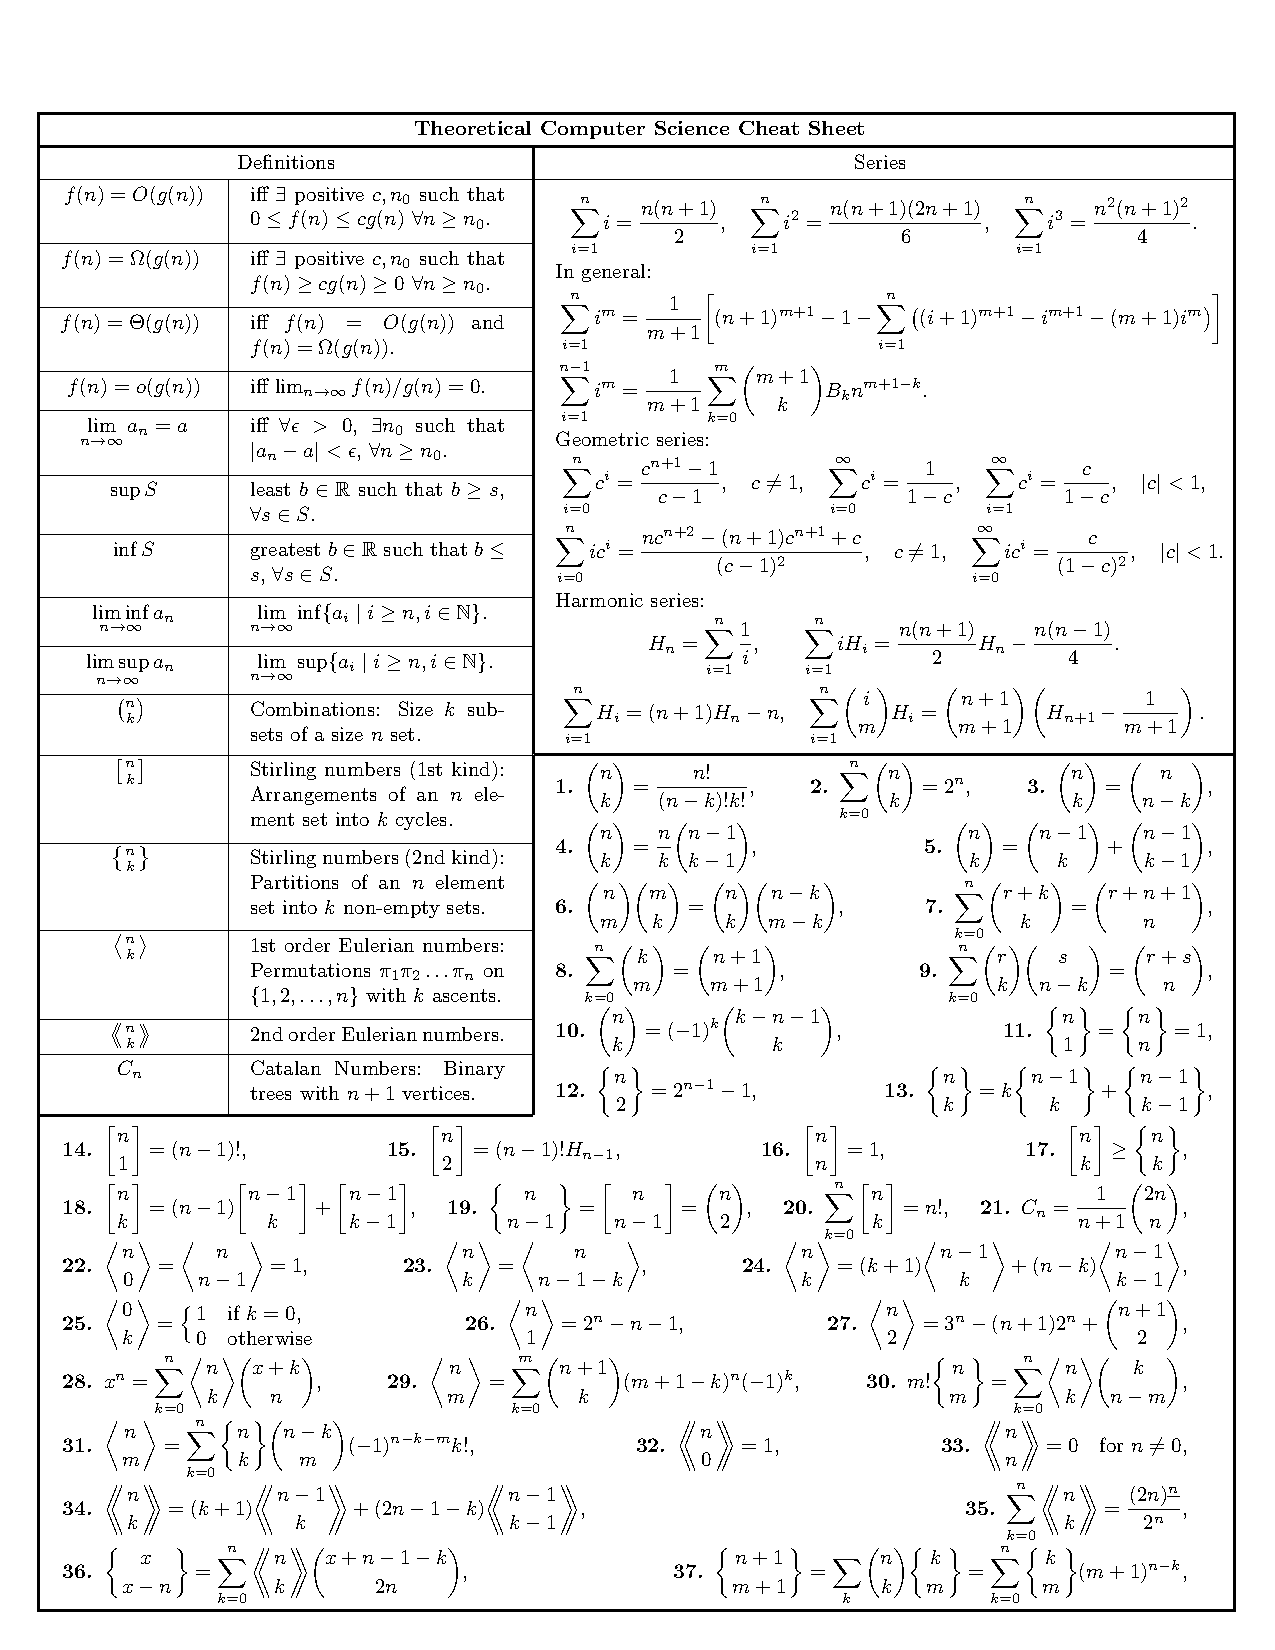
\includepdf[pages=-]{source/cheat.pdf}

%\newpage
%\section{source/others}

\end{document}
